\documentclass[conference,a4paper]{IEEEtran}
\IEEEoverridecommandlockouts
\usepackage{cite}
\usepackage{amsmath,amssymb,amsfonts}
\usepackage{graphicx}
\usepackage{textcomp}
\usepackage{xcolor}
\usepackage{booktabs}
\usepackage{multirow}
\usepackage{tikz}
\usetikzlibrary{shapes.geometric, arrows.meta, positioning, calc, shadows}

\def\BibTeX{{\rm B\kern-.05em{\sc i\kern-.025em b}\kern-.08em
    T\kern-.1667em\lower.7ex\hbox{E}\kern-.125emX}}

\begin{document}

% -----------------------------------------------------------------------
% TITLE
% -----------------------------------------------------------------------
\title{HIKARI: A Multi-Stage Vision-Language Prototype\\
with RAG-in-Training for Medical Lesion Diagnosis\\
and Clinical Recommendations}

% -----------------------------------------------------------------------
% AUTHORS
% -----------------------------------------------------------------------
\author{
\IEEEauthorblockN{1\textsuperscript{st} Watin Promfiy}
\IEEEauthorblockA{\textit{Department of Information Technology}\\
\textit{King Mongkut's Institute of}\\
\textit{Technology Ladkrabang}\\
Bangkok, Thailand}
\and
\IEEEauthorblockN{2\textsuperscript{nd} Pawitra Boonprasart}
\IEEEauthorblockA{\textit{Department of Information Technology}\\
\textit{King Mongkut's Institute of}\\
\textit{Technology Ladkrabang}\\
Bangkok, Thailand}
\and
\IEEEauthorblockN{3\textsuperscript{rd} Given Name Surname}
\IEEEauthorblockA{\textit{Department of Information Technology}\\
\textit{King Mongkut's Institute of}\\
\textit{Technology Ladkrabang}\\
Bangkok, Thailand}
}

\maketitle

% -----------------------------------------------------------------------
% ABSTRACT
% -----------------------------------------------------------------------
\begin{abstract}
We present HIKARI (\textbf{H}ealthcare-oriented \textbf{I}ntelligent
\textbf{K}nowledge-\textbf{A}ugmented \textbf{R}etrieval and
\textbf{I}nference system), a prototype multi-stage Vision-Language Model
(VLM) pipeline for medical lesion diagnosis and clinical caption generation.
Validated on skin dermatology as a representative domain, the architecture
is designed to generalize across oral mucosal disease, fundus lesions, and
other medical imaging modalities.
Retrieval-Augmented Generation (RAG) provides visual few-shot context at
inference time, yet a train-inference distribution gap persists when the
model is fine-tuned on single images.
We propose \textbf{RAG-in-Training}, which incorporates retrieved reference
images into every training sample, enabling the VLM to exploit reference
context at inference.
Built on a three-stage cascaded Low-Rank Adaptation (LoRA) fine-tuning
pipeline using Qwen3-VL-8B-Thinking on the SkinCAP dataset (10 disease
classes, 99 validation samples), HIKARI achieves 85.86\% classification accuracy, surpassing the
single-image fine-tuned (FT) baseline by 11.86~pp (74.00\%) and
inference-only RAG by 6.06~pp (79.80\%).
We further show that merging adapter weights before switching tasks
(\textbf{Merged-Init}) yields a 3$\times$ BLEU-4 gain for caption
generation (9.82 $\rightarrow$ 29.33).
\end{abstract}

\begin{IEEEkeywords}
medical lesion classification, retrieval-augmented generation,
vision-language model, LoRA fine-tuning, multi-stage training,
clinical caption generation, dermoscopy, HIKARI
\end{IEEEkeywords}

% -----------------------------------------------------------------------
% I. INTRODUCTION
% -----------------------------------------------------------------------
\section{Introduction}

Medical lesion diagnosis from clinical images is a key step in many
specialist workflows.  For skin dermatology, dermoscopy-based
classification has achieved competitive performance on standard benchmarks
such as HAM10000~\cite{tschandl2018} and ISIC~\cite{codella2019}, yet
fine-grained discrimination among visually similar inflammatory
diseases---psoriasis, lupus erythematosus, and lichen planus---remains
difficult due to limited labeled data per class and subtle inter-class
morphological differences.  Analogous challenges arise in oral mucosal
disease~\cite{zhang2025oralgpt}, diabetic retinopathy, and
colonoscopy polyp grading.

We present \textbf{HIKARI} (\textbf{H}ealthcare-oriented
\textbf{I}ntelligent \textbf{K}nowledge-\textbf{A}ugmented
\textbf{R}etrieval and \textbf{I}nference system), a prototype
multi-stage vision-language pipeline addressing three interrelated
problems: (1) fine-grained lesion classification,
(2) structured clinical caption generation, and (3) the
train-inference distribution gap introduced when RAG is applied only
at inference time.
The architecture is validated on skin lesion data as a first application;
the same pipeline can be directly applied to other medical lesion domains
by replacing the RAG index.

VLMs such as Qwen3-VL~\cite{qwen2023} offer rich visual representations;
however, standard single-image fine-tuning leaves the model unable to
leverage retrieved references at inference.
RAG~\cite{lewis2020} alone is insufficient: seven frontier VLMs tested
with identical retrieved context score only 12.87--50.51\%, confirming
that without RAG-aware training, reference injection does not help.

HIKARI addresses this distribution gap with three contributions:

\begin{itemize}
  \item \textbf{RAG-in-Training:} retrieved reference images are
        included in every training sample, teaching the VLM to
        actively leverage visual comparisons (74.00\%
        $\rightarrow$ 85.86\%).
  \item \textbf{Hybrid RAG encoder evaluation:} five image/text encoder
        combinations are benchmarked, revealing image-dominant weighting
        ($\alpha{=}0.9$) is optimal for dermoscopy retrieval.
  \item \textbf{Merged-Init finding:} merging prior-stage LoRA adapters
        into base weights before a new task yields 3$\times$ BLEU-4
        improvement in caption generation (9.82 $\rightarrow$ 29.33).
\end{itemize}

% -----------------------------------------------------------------------
% II. RELATED WORK
% -----------------------------------------------------------------------
\section{Related Work}

\textbf{Medical lesion classification.}
Esteva et al.~\cite{esteva2017} demonstrated dermatologist-level
performance using CNNs on a large skin lesion dataset.  Transformer-based models and contrastive pretraining have since improved
accuracy on the ISIC challenge~\cite{codella2019}, yet VLM-based approaches
beyond zero-shot prompting remain underexplored for fine-grained dermoscopy.

\textbf{RAG for medical imaging.}
Lewis et al.~\cite{lewis2020} introduced RAG for knowledge-intensive NLP
tasks. Multi-modal extensions have shown gains in medical visual question
answering~\cite{jin2023medcpt}, yet retrieval at inference without
corresponding training-time exposure creates a distribution gap that
our work directly targets.

\textbf{Multi-stage LoRA fine-tuning.}
Hu et al.~\cite{hu2022lora} introduced Low-Rank Adaptation (LoRA) for
efficient VLM fine-tuning; cascaded application can cause catastrophic
interference when adapters are reused across tasks.
OralGPT~\cite{zhang2025oralgpt} demonstrates a two-stage VLM pipeline
for oral mucosal disease, confirming sequential task specialization
outperforms joint training in low-data domains.
Our Merged-Init strategy eliminates this interference by absorbing
prior-stage adapters into full-rank base weights before attaching fresh
LoRA for each new task.

% -----------------------------------------------------------------------
% III. METHODOLOGY
% -----------------------------------------------------------------------
\section{Methodology}

\subsection{Three-Stage Cascaded Fine-Tuning}

Our pipeline progressively specializes a Qwen3-VL-8B-Thinking backbone
across three stages (Fig.~\ref{fig:pipeline}).

\textbf{Stage 1} classifies skin lesions into four coarse groups:
Inflammatory \& Autoimmune, Benign Tumors \& Nevi, Malignant Tumors, and
Acne \& Follicular Disorders, achieving \textbf{88.68\%} accuracy.
The merged Stage~1 weights initialize Stage~2, providing
dermoscopy-adapted representations (+4.6 pp over base-model initialization).

\textbf{Stage 2} fine-tunes for 10-class disease classification.
Both stages share LoRA hyperparameters: rank $r{=}16$, scaling
$\alpha_{LoRA}{=}32$, dropout${=}0$, learning rate $2{\times}10^{-4}$,
3 epochs, AdamW 8-bit, effective batch size 8
(2 per device $\times$ gradient accumulation 4), trained on an
NVIDIA RTX~5070~Ti (15.92\,GB VRAM).
A custom \texttt{MemoryCleanupCallback} clears the CUDA cache every
100 steps, eliminating VRAM fragmentation and yielding a
\textbf{32$\times$ training speedup}.

\textbf{Stage 3} fine-tunes for clinical caption generation from the
merged Stage~2 model (Section~\ref{sec:mergedinit}).

% -----------------------------------------------------------------------
% FULL-WIDTH ARCHITECTURE DIAGRAM
% -----------------------------------------------------------------------
\begin{figure*}[t]
\centering
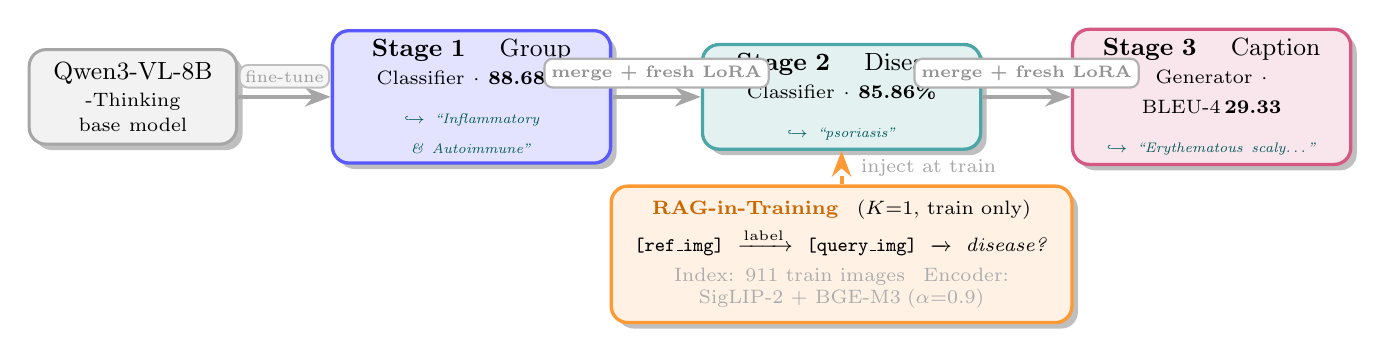
\begin{tikzpicture}[
  base/.style={
    rectangle, rounded corners=6pt,
    draw=gray!70, fill=gray!10, line width=1.1pt,
    text width=2.4cm, align=center,
    minimum height=1.2cm, font=\small, drop shadow},
  s1box/.style={
    rectangle, rounded corners=6pt,
    draw=blue!65, fill=blue!11, line width=1.2pt,
    text width=3.3cm, align=center,
    minimum height=1.2cm, font=\small, drop shadow},
  s2box/.style={
    rectangle, rounded corners=6pt,
    draw=teal!70, fill=teal!11, line width=1.2pt,
    text width=3.3cm, align=center,
    minimum height=1.2cm, font=\small, drop shadow},
  s3box/.style={
    rectangle, rounded corners=6pt,
    draw=purple!65, fill=purple!10, line width=1.2pt,
    text width=3.3cm, align=center,
    minimum height=1.2cm, font=\small, drop shadow},
  ragbox/.style={
    rectangle, rounded corners=6pt,
    draw=orange!80, fill=orange!10, line width=1.2pt,
    text width=5.5cm, align=center, font=\scriptsize, inner sep=5pt,
    drop shadow},
  mergebadge/.style={
    rectangle, rounded corners=3pt,
    draw=gray!60, fill=white, line width=0.8pt,
    font=\fontsize{6.5}{7.5}\selectfont\bfseries,
    text=gray!85, inner sep=2.5pt},
  ftbadge/.style={
    rectangle, rounded corners=3pt,
    draw=gray!50, fill=gray!8, line width=0.7pt,
    font=\fontsize{6.5}{7.5}\selectfont,
    text=gray!75, inner sep=2pt},
  arrowmain/.style={-Stealth, line width=1.4pt, draw=gray!70},
  arrowrag/.style={-Stealth, line width=1.4pt, draw=orange!80, dashed},
  lbl/.style={font=\scriptsize, text=gray!70},
]

%% ---- Main pipeline (horizontal) ----
\node[base] (base) at (0, 0) {%
  Qwen3-VL-8B\\[-1pt]
  {\scriptsize -Thinking}\\[-2pt]
  {\scriptsize base model}};

\node[s1box] (s1) at (4.3, 0) {%
  \textbf{Stage 1} \quad Group\\[-1pt]
  {\scriptsize Classifier $\cdot$ \textbf{88.68\%}}\\[3pt]
  {\tiny\color{teal!70!black}%
   $\hookrightarrow$ \textit{``Inflammatory \& Autoimmune''}}};

\node[s2box] (s2) at (9.0, 0) {%
  \textbf{Stage 2} \quad Disease\\[-1pt]
  {\scriptsize Classifier $\cdot$ \textbf{85.86\%}}\\[3pt]
  {\tiny\color{teal!70!black}%
   $\hookrightarrow$ \textit{``psoriasis''}}};

\node[s3box] (s3) at (13.7, 0) {%
  \textbf{Stage 3} \quad Caption\\[-1pt]
  {\scriptsize Generator $\cdot$ BLEU-4\,\textbf{29.33}}\\[3pt]
  {\tiny\color{teal!70!black}%
   $\hookrightarrow$ \textit{``Erythematous scaly\ldots''}}};

%% ---- Pipeline arrows ----
\draw[arrowmain] (base.east) --
  node[ftbadge, above=3pt]{fine-tune} (s1.west);

\draw[arrowmain] (s1.east) --
  node[mergebadge, above=3pt]{\textbf{merge} + fresh LoRA} (s2.west);

\draw[arrowmain] (s2.east) --
  node[mergebadge, above=3pt]{\textbf{merge} + fresh LoRA} (s3.west);

%% ---- RAG-in-Training component (below Stage 2) ----
\node[ragbox] (rag) at (9.0, -2.0) {%
  \textbf{\textcolor{orange!80!black}{RAG-in-Training}}
  \enspace ($K{=}1$, train only)\\[2pt]
  \texttt{[ref\_img]}
    \;$\xrightarrow{\text{label}}$\;
  \texttt{[query\_img]}
    \;$\xrightarrow{}$\;
  \textit{disease?}\\[3pt]
  {\color{gray!65}%
   Index: 911 train images \enspace
   Encoder: SigLIP-2 + BGE-M3\;($\alpha{=}0.9$)}};

\draw[arrowrag] (rag.north) --
  node[lbl, right=3pt]{inject at train} (s2.south);

\end{tikzpicture}
\caption{HIKARI three-stage pipeline. \textbf{Merged-Init} (white badges
on arrows) absorbs LoRA adapters into base weights before each stage
transition, preventing catastrophic interference. \textbf{RAG-in-Training}
(orange, train only) injects one retrieved reference image per Stage~2
sample. Teal text shows example outputs at each stage.}
\label{fig:pipeline}
\end{figure*}

\subsection{RAG-in-Training}
\label{sec:rag}

\textbf{Hybrid RAG index.}
For each training image we pre-compute embeddings using a hybrid encoder
(image encoder + text encoder on clinical captions).
The index is built from all 911 training images; validation images are
excluded to prevent data leakage.  The retrieval score is:
\begin{equation}
s(q,i) = \alpha\,\cos\!\bigl(\mathbf{e}^{img}_{q},\mathbf{e}^{img}_{i}\bigr)
        + (1{-}\alpha)\,\cos\!\bigl(\mathbf{e}^{txt}_{q},\mathbf{e}^{txt}_{i}\bigr),
\label{eq:score}
\end{equation}
where $\alpha$ controls image-to-text weight ($\alpha{=}1$: image only;
$\alpha{=}0$: text only).
We evaluate five encoder configurations (Table~\ref{tab:encoders}).

\textbf{Training sample format.}
Each Stage~2 sample includes $K{=}1$ retrieved reference ($K{=}3$
exhausts the 15.92\,GB VRAM budget on a single RTX~5070~Ti):
\begin{center}
{\footnotesize\ttfamily\raggedright\setlength{\baselineskip}{1.3\baselineskip}
Here are similar reference cases for context:\\
$\langle$ref\_img$\rangle$\ \ Reference 1: psoriasis\\
Now, identify the disease in this new image:\\
$\langle$query\_img$\rangle$\ \ What skin disease is shown in this image?\\
\textrm{$\hookrightarrow$ \textit{Answer:} \texttt{psoriasis}}
}
\end{center}
Reference embeddings are pre-computed before loading Qwen3-VL.

\textbf{Output parsing.}
Raw outputs are parsed by (1) stripping \texttt{<think>...</think>}
blocks (Qwen3-VL-8B-Thinking emits chain-of-thought reasoning tokens),
(2) anchor extraction (e.g., \texttt{Diagnosis:}), and
(3) fuzzy word-overlap matching (Jaccard similarity ${\geq}0.91$) against 10 disease
name strings.  Unmatched outputs are classified as ``Unknown'' and
counted incorrect.

\subsection{Merged-Init for Task Switching}
\label{sec:mergedinit}

\textbf{Way 1 (Checkpoint Init)} continues fine-tuning the same Stage~2
LoRA adapters on caption data; caption gradients overwrite disease
representations in the shared adapters, causing catastrophic
interference.  \textbf{Way 2 (Merged-Init)} first merges Stage~2
(LoRA $\rightarrow$ full weights), then attaches fresh zero-initialized
adapters for caption training; disease knowledge is permanently encoded
in the frozen base weights.  Way~2 achieves BLEU-4\,=\,29.33 versus
9.82 for Way~1 (Table~\ref{tab:caption}).


% -----------------------------------------------------------------------
% IV. EXPERIMENTS
% -----------------------------------------------------------------------
\section{Experiments}

\subsection{Dataset and Setup}

\textbf{SkinCAP}~\cite{mendez2022} contains 4,000 dermatological images
with disease labels and clinical captions.  We filter to 10 disease
classes across four groups (1,010 images) with a stratified split:
911 train / 99 validation (locked; never regenerated).  Rare classes
are square-root oversampled; images are resized to $672{\times}672$ px
using Lanczos filtering.

Disease classes include: psoriasis, lupus erythematosus,
lichen planus, scleroderma, photodermatoses, sarcoidosis
(Inflammatory \& Autoimmune group); melanocytic nevi (Benign group);
Squamous Cell Carcinoma In Situ (SCCIS), Basal Cell Carcinoma (BCC)
(Malignant group); and acne vulgaris (Acne group).

\subsection{RAG Encoder Comparison}

Table~\ref{tab:encoders} compares five encoder combinations on the
\textit{Cascaded FT} model (inference-only RAG).
R2 (SigLIP-2~\cite{zhai2023} + BGE-M3~\cite{chen2024bge}) at
$\alpha{=}0.9$ achieves the best accuracy and is selected for
RAG-in-Training.  Image-dominant weighting ($\alpha{=}0.9$)
consistently outperforms balanced weighting ($\alpha{=}0.5$) because
dermoscopy diagnosis is predominantly visual; clinical text captions
at equal weight introduce retrieval noise.

\begin{table}[!ht]
\caption{RAG Encoder Comparison -- Cascaded FT model, Prompt P0
         (99 val samples)}
\label{tab:encoders}
\begin{center}
\setlength{\tabcolsep}{4pt}
\begin{tabular}{clcc}
\toprule
\textbf{ID} & \textbf{Encoder (Image + Text)} & \textbf{$\alpha$=0.5} & \textbf{Best Acc.} \\
\midrule
R0 & CLIP ViT-B/32~\cite{radford2021} + None & 72.73\%  & 72.73\% \\
R1 & CLIP + ClinicalBERT          & 69.70\%  & 71.72\% ($\alpha{=}0.9$) \\
\textbf{R2} & \textbf{SigLIP-2 + BGE-M3} & \textbf{74.75\%} & \textbf{79.80\% ($\alpha{=}0.9$)} \\
R3 & Jina-CLIP-v2 + MedCPT       & 66.67\%  & 78.79\% ($\alpha{=}0.7$) \\
R4 & Nomic Vision + Nomic Text   & 67.68\%  & 72.73\% ($\alpha{=}0.9$) \\
\bottomrule
\end{tabular}
\end{center}
\end{table}

\subsection{Main Classification Results}

Table~\ref{tab:main} reports classification accuracy on the locked
99-sample validation set.  Seven frontier VLMs tested with CLIP-retrieved
(R0) reference context but no fine-tuning all score 12.87--50.51\%,
confirming that without RAG-aware training, reference injection alone
does not improve performance.

\textbf{HIKARI with RAG-in-Training} achieves 85.86\%, surpassing
inference-only RAG (\textit{Cascaded FT}, R2 $\alpha{=}0.9$, 79.80\%)
by 6.06 pp and the single-image FT baseline (74.00\%) by 11.86 pp.
The \textit{2-Stage Cascade FT} model, when tested with RAG at inference,
scores only 59.38\%, further confirming that reference context only
helps when the model is trained to exploit it.  Notably, CLIP (R0) at
inference outperforms the R2 encoder used during training by 3.03 pp
(85.86\% vs.\ 82.83\%), showing that RAG-in-Training imparts a
generalizable \textit{compare-and-decide} skill---the retrieval encoder
can be swapped without retraining.

\begin{table}[!ht]
\caption{Main Classification Results (99 val samples, all author-evaluated).
         Zero-shot models receive CLIP (R0) context but no fine-tuning.}
\label{tab:main}
\begin{center}
\setlength{\tabcolsep}{3pt}
\begin{tabular}{lccc}
\toprule
\textbf{Model} & \textbf{RAG Train} & \textbf{RAG Infer.} & \textbf{Acc.} \\
\midrule
\multicolumn{4}{l}{\textit{Zero-Shot Frontier Models (no fine-tuning)}} \\
LLaMA-4-Scout-17B             & --      & R0   & 12.87\% \\
LLaMA-4-Maverick-17B          & --      & R0   & 12.87\% \\
Gemini-2.5-Flash              & --      & R0   & 25.74\% \\
Gemini-3.1-Pro                & --      & R0   & 23.23\% \\
Gemini-2.5-Pro                & --      & R0   & 30.69\% \\
Qwen3-VL-8B                   & --      & R0   & 33.33\% \\
Qwen2.5-VL-7B~\cite{qwen2023} & --      & R0   & 50.51\% \\
\midrule
\multicolumn{4}{l}{\textit{Domain Fine-Tuned (No Training RAG)}} \\
Single-Image FT               & --      & --   & 74.00\% \\
2-Stage Cascade FT            & --      & R0   & 59.38\% \\
\midrule
\multicolumn{4}{l}{\textit{Inference-Only RAG (Cascaded FT)}} \\
Cascaded FT (R2, $\alpha{=}0.5$)       & --      & R2   & 74.75\% \\
Cascaded FT (R2, $\alpha{=}0.9$)       & --      & R2   & 79.80\% \\
\midrule
\multicolumn{4}{l}{\textit{RAG-in-Training (Ours)}} \\
RAG-in-Training (R2 train, R2) & R2 K=1 & R2   & 82.83\% \\
\textbf{RAG-in-Training (R2 train, R0)} & \textbf{R2 K=1} & \textbf{R0} & \textbf{85.86\%} \\
\bottomrule
\end{tabular}
\end{center}
\end{table}

\subsection{Per-Disease Analysis}

RAG-in-Training strictly improves 5 of 10 diseases and matches 3 others,
with psoriasis showing the largest gain (+38.5~pp, 61.5\%$\rightarrow$100\%)
and five diseases reaching 100\% sensitivity (psoriasis, BCC, melanocytic
nevi, SCCIS, acne vulgaris).  Sarcoidosis drops sharply
(57.1\%$\rightarrow$14.3\%) because retrieved references are visually
heterogeneous, biasing prediction toward the reference label; contrastive
hard-negative training is identified as the primary mitigation.

\subsection{Stage 3 Caption Generation Ablation}

Table~\ref{tab:caption} validates the Merged-Init strategy.
Way~2 achieves BLEU-4\,=\,29.33, three times higher than Way~1 (9.82),
confirming that absorbing prior-stage adapters into the base model
prevents catastrophic interference when switching tasks.

\begin{table}[!ht]
\caption{Stage 3 Caption Ablation: Checkpoint vs.\ Merged Init}
\label{tab:caption}
\begin{center}
\setlength{\tabcolsep}{4pt}
\begin{tabular}{lcccc}
\toprule
\textbf{Init} & \textbf{B-1} & \textbf{B-2} & \textbf{B-4} & \textbf{R-1} \\
\midrule
Checkpoint      & 29.22 & 18.65 & 9.82  & 38.9 \\
\textbf{Merged} & \textbf{42.22} & \textbf{35.19} & \textbf{29.33} & \textbf{53.6} \\
\bottomrule
\multicolumn{5}{l}{\scriptsize B-$n$: BLEU-$n$; R-1: ROUGE-1}
\end{tabular}
\end{center}
\end{table}

\subsection{Attention Map Analysis}

We average per-head attention over the last four transformer layers
(prefill, last-input token to all \texttt{<|image\_pad|>} positions)
to produce a patch saliency map upsampled to full resolution.

\begin{figure}[!ht]
\centering

\includegraphics[width=\columnwidth]{melanocytic_nevi_2_comparison.png}\\[2pt]

\includegraphics[width=\columnwidth]{basal_cell_carcinoma_3_comparison.png}
\caption{Attention maps for melanocytic nevi (top) and BCC (bottom).
Each row: \textbf{Original}; \textbf{Base} Qwen3-VL-8B (diffuse, lesion
unlocalised); \textbf{HIKARI} (concentrated on the pigmented lesion for
nevi; on the annotated nodule for BCC). Warmer colours = higher attention.}
\label{fig:gradcam}
\end{figure}

Fig.~\ref{fig:gradcam} shows the base model distributes attention diffusely,
while HIKARI concentrates on clinically discriminating regions---the pigmented
network and border for nevi; the annotated nodular lesion for BCC---providing
an interpretability signal consistent with clinical differential diagnosis.

% -----------------------------------------------------------------------
% V. DISCUSSION
% -----------------------------------------------------------------------
\section{Discussion}

The 6.06~pp gain over inference-only RAG confirms that reference context
only helps when the model is \textit{trained to use it}: repeated
(reference, label, query) tuples build a ``compare-and-decide'' skill that
transfers to unseen retrievers---CLIP at inference outperforms the
SigLIP+BGE-M3 encoder used during training by 3.03~pp, demonstrating
encoder-agnostic generalisation.
The 3$\times$ BLEU-4 gain from Merged-Init follows the same principle:
Way~2 locks disease knowledge in full-rank base weights before attaching
fresh adapters for caption training, eliminating gradient interference---a
guideline applicable to any multi-task LoRA pipeline.

\textbf{Limitations.}
The 1,010-image SkinCAP subset (80--130 samples per rare class) limits
statistical power; each validation sample corresponds to $\approx$1~pp,
making low-count results such as sarcoidosis (14.3\%) fragile.
Contrastive hard-negative training and higher-$K$ retrieval on multi-GPU
are the most promising next steps.
All results are on a single domain; generalisation to HAM10000, ISIC, oral
mucosal disease, and fundus imaging remains future work.

% -----------------------------------------------------------------------
% VI. CONCLUSION
% -----------------------------------------------------------------------
\section{Conclusion}

We presented HIKARI, a three-stage VLM prototype for medical lesion
diagnosis and clinical caption generation, first validated on skin
dermatology data.  \textbf{RAG-in-Training} closes the train-inference
distribution gap and achieves 85.86\% accuracy on SkinCAP, outperforming
both the single-image FT baseline (+11.86 pp) and inference-only RAG
(+6.06 pp).  Author-evaluated zero-shot tests of seven frontier VLMs
confirm that even state-of-the-art models fail to exploit reference
context without RAG-aware training (12.87--50.51\%).
\textbf{Merged-Init} provides a practical guideline for multi-stage
LoRA pipelines, yielding a 3$\times$ BLEU-4 improvement
(9.82 $\rightarrow$ 29.33), and makes the approach accessible on a
single consumer GPU.

The HIKARI architecture is domain-agnostic: by replacing the RAG index
with an oral lesion database, a fundus atlas, or an endoscopy case
library, the same three-stage pipeline can be applied to any medical
lesion modality---a direction we are actively pursuing.

% -----------------------------------------------------------------------
% ACKNOWLEDGMENT
% -----------------------------------------------------------------------
\section*{Acknowledgment}

\textit{AI Disclosure (IEEE Policy):} Claude Sonnet~4.6 (Anthropic) was
used to assist with grammar, phrasing, and logical flow in the Abstract,
Introduction, Related Work, Discussion, and Conclusion sections.
All experimental results, methodology, code implementation, numerical
values, and scientific conclusions are entirely the work of the authors.

% -----------------------------------------------------------------------
% REFERENCES
% -----------------------------------------------------------------------
\begin{thebibliography}{00}

\bibitem{tschandl2018}
P. Tschandl, C. Rosendahl, and H. Kittler,
``The HAM10000 dataset,''
\textit{Scientific Data}, vol. 5, p. 180161, 2018.

\bibitem{codella2019}
N. Codella et al.,
``Skin lesion analysis toward melanoma detection 2018 (ISIC),''
\textit{arXiv:1902.03368}, 2019.

\bibitem{esteva2017}
A. Esteva et al.,
``Dermatologist-level classification of skin cancer with deep neural
networks,''
\textit{Nature}, vol. 542, pp. 115--118, 2017.

\bibitem{hu2022lora}
E. J. Hu et al.,
``LoRA: Low-rank adaptation of large language models,''
in \textit{Proc. ICLR}, 2022.

\bibitem{lewis2020}
P. Lewis et al.,
``Retrieval-augmented generation for knowledge-intensive NLP tasks,''
in \textit{Proc. NeurIPS}, 2020, pp. 9459--9474.

\bibitem{radford2021}
A. Radford et al.,
``Learning transferable visual models from natural language supervision,''
in \textit{Proc. ICML}, 2021, pp. 8748--8763.

\bibitem{zhai2023}
X. Zhai, B. Mustafa, A. Kolesnikov, and L. Beyer,
``Sigmoid loss for language image pre-training,''
in \textit{Proc. ICCV}, 2023, pp. 11975--11986.

\bibitem{chen2024bge}
J. Chen et al.,
``BGE M3-embedding: Multi-lingual, multi-functionality,
multi-granularity text embeddings,''
\textit{arXiv:2309.07597}, 2024.

\bibitem{jin2023medcpt}
Q. Jin et al.,
``MedCPT: Contrastive pre-trained transformers with large-scale PubMed
search logs for zero-shot biomedical information retrieval,''
\textit{Bioinformatics}, vol. 39, no. 11, 2023.

\bibitem{mendez2022}
D. M\'{e}ndez et al.,
``SkinCAP: A multi-modal dermatology dataset annotated with rich medical
captions,''
in \textit{Proc. NeurIPS Datasets and Benchmarks}, 2022.

\bibitem{qwen2023}
J. Bai et al.,
``Qwen-VL: A versatile vision-language model for understanding,
localization, text reading, and beyond,''
\textit{arXiv:2308.12966}, 2023.

\bibitem{zhang2025oralgpt}
J. Zhang, B. Du, Y. Miao, D. Sun, and X. Cao,
``OralGPT: A two-stage vision-language model for oral mucosal disease
diagnosis and description,''
\textit{arXiv:2510.13911}, 2025.

\end{thebibliography}

\end{document}
